% 切空间：曲面片、切平面与切向量
\documentclass[border=4pt]{standalone}
\usepackage{tikz}
\usetikzlibrary{arrows.meta}
\usepackage{amsmath,amssymb}
\definecolor{fillA}{rgb}{0.45,0.45,0.45}
\definecolor{fillB}{rgb}{0.72,0.72,0.72}
\begin{document}
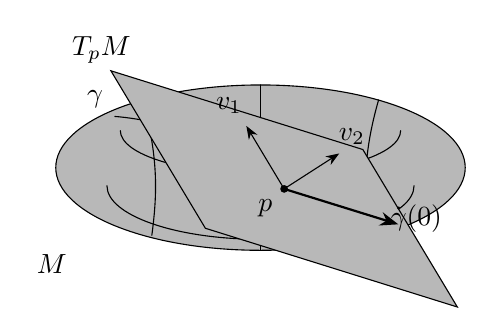
\begin{tikzpicture}[>=Stealth, line cap=round]
% 曲面片（带坐标曲线）
\draw[fill=fillB] (3.0,1.95) ellipse (2.6 and 1.05);
\draw (1.5,2.81) .. controls (1.72,2.05) and (1.68,1.55) .. (1.62,1.09);
\draw (3.0,3.0) -- (3.0,0.9);
\draw (4.5,2.81) .. controls (4.28,2.05) and (4.32,1.55) .. (4.38,1.09);
\draw (1.22,2.42) arc (180:360:1.78 and 0.55);
\draw (1.05,1.72) arc (180:360:1.95 and 0.68);
% 过 p 的曲线 gamma
\draw plot[smooth, tension=0.85] coordinates {(1.15,2.6) (2.2,2.35) (3.3,1.68) (4.4,1.35) (4.75,1.3)};
\node at (0.9,2.82) {$\gamma$};
% 切平面 T_pM
\draw[fill=fillB] (1.1,3.18) -- (2.3,1.18) -- (5.5,0.18) -- (4.3,2.18) -- cycle;
% 切向量
\draw[->, thick] (3.3,1.68) -- (4.75,1.23);
\node at (4.98,1.3) {$\dot\gamma(0)$};
\draw[->] (3.3,1.68) -- (2.82,2.48);
\node at (2.6,2.74) {$v_1$};
\draw[->] (3.3,1.68) -- (4.0,2.13);
\node at (4.16,2.34) {$v_2$};
% 点与标注
\fill (3.3,1.68) circle (1.4pt);
\node at (3.06,1.44) {$p$};
\node at (0.98,3.44) {$T_pM$};
\node at (0.35,0.72) {$M$};
\end{tikzpicture}
\end{document}
